%Om filen typsätts som del av hela rapporten så finns \master definierat i början och ingen \begin{document} och \end{document} får finnas, men för att kunna typsätta filen för sig är dem ett måste! \newcommand{\master}{} krävs i början på huvudrapporten!

\ifdefined\master
\else
	\documentclass[twocolumn]{article}
\usepackage{graphicx}
\usepackage{float} %gör så att man kan placera bilder exakt mha [H]
	%\input{../preamble}
	\begin{document}
\fi
%text goes here!
\section{Lab demonstration}
To demonstrate the functionality of the program an easy lab-assignment was performed. A RC-circuit was connected like figure \ref{fig:RCcircuit}, the circuit is a low-pass filter with the cutoff frequency at $f=1.5~kHz$. 
	\begin{figure}[h]
	\centering
		\fbox{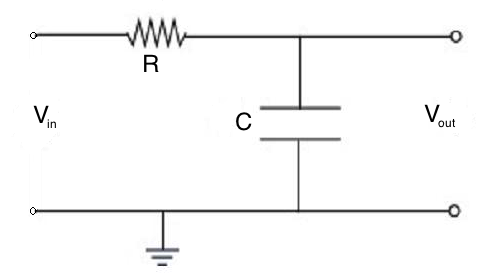
\includegraphics[width=4cm]{Figure/rc-circuit}}
		\caption{RC-circuit}
		\label{fig:RCcircuit}
	\end{figure}

Start with connecting the oscilloskop, multimeter, function- and voltage generator to the computer using the GIPB-port, you need to check that every device have a different GPIB-address to be sure that all will work.  

\subsection{Assignment 1}
The first assignment is about looking at the difference between the in- and out-signal. Set the function generator to a frequency at $1~kHz$ and the amplitude to $3~V$ you also need to add the GIPB-address of the function generator and the oscilloskop. Click at \emph{Set} bottom in the function generator panel and select \emph{oscilloskop picture} in the popup-menu at the out panel an then. Now you need to add the GPIB-address to the oscilloskop and click start to get a picture from the oscilloskop. Figure \ref{oscilloskopPicture} shows a picture from the oscilloskop whit the settings mentioned above. 
	\begin{figure}[H]
	\centering
		\fbox{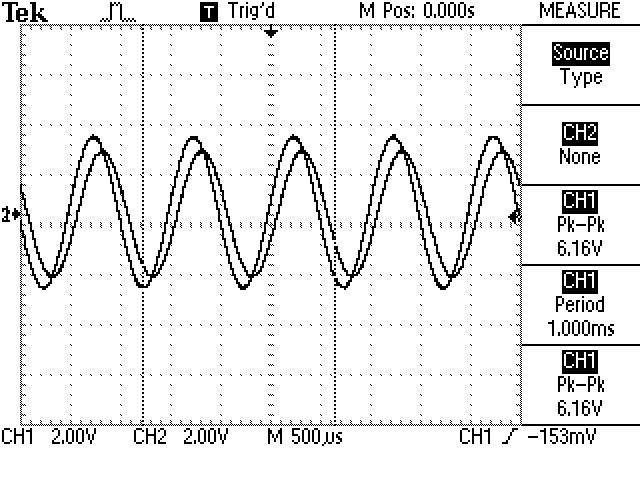
\includegraphics[width=6cm]{Figure/screenshot.png}}
		\caption{Oscilloscope picture.}
		\label{oscilloskopPicture}
	\end{figure}

Now we wont to use the export function to implement the figure in a report. By selecting the \emph{LaTeX} alternate in export popup-menu, your able to change the title and  figure labels  by typing the wonted label name in the \emph{X-Label} and \emph{Y-Label} text boxes, the figure title is chanced by typing in the \emph{Title} text box. You can also set the LaTeX figure caption and reference label by typing in the \emph{Label} and \emph{Caption} text boxes. Than it's jest to type a figure name and click \emph{export} and chose a location for the file to be saved.

\subsection{Assignment 2}
Connect the multimeter to measuring the voltage over the resistor. Change the output bar to multimeter, select the \emph{Voltage [AC]} in the measuring popup-menu, add the GPIB-address for the multimeter and press start button. Now you will see the multimeter display in the black text box in the out-panel. By clicking the \emph{Stop}-button you stop the multimeter and you can save the data in a .mat file and also present the measerment in a stem-graph by saving the figure. The generated stem-graph is presented in figure \ref{stem} 
	\begin{figure}[H]
	\centering
		\fbox{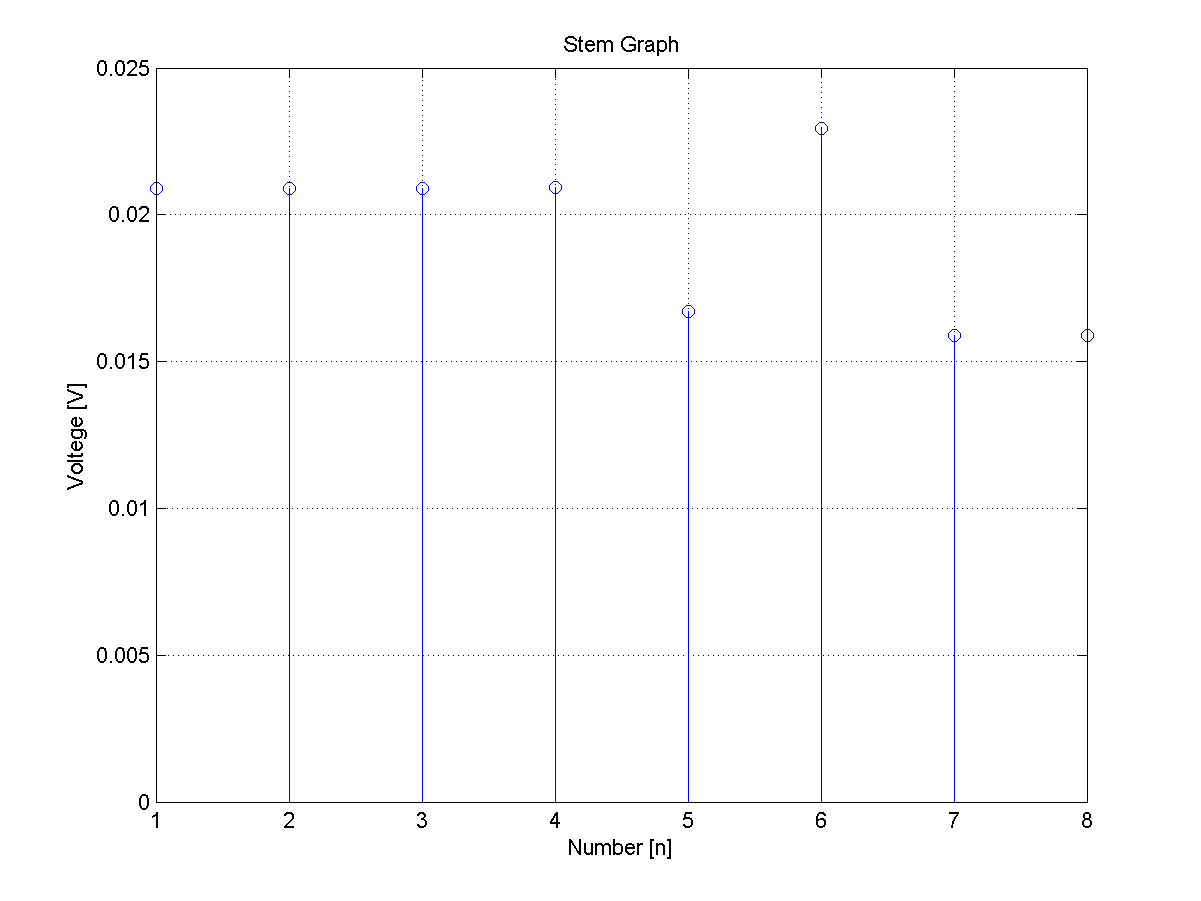
\includegraphics[width=6cm]{Figure/stem.png}}
		\caption{stem graph}
		\label{stem}
	\end{figure}

\subsection{Assignment 3}
Now move the multimeter probes to measuring the out voltage and change to \emph{frequency sweep} in the input popup-menu and set the start, end frequency to $0~Hz$ and $3000~Hz$ and the step length to $100~Hz$ use \emph{Sine} as waveform with an amplitude at $3~V$ and click \emph{Start sweep}. This will take some time.\\
\\
The generated bode graph figure \ref{bode} can be exported to a Word-document in the same way as the LaTeX export, the generated frequency and voltage can also be saved for other use in MATLABs workspace. 
	\begin{figure}[H]
	\centering
		\fbox{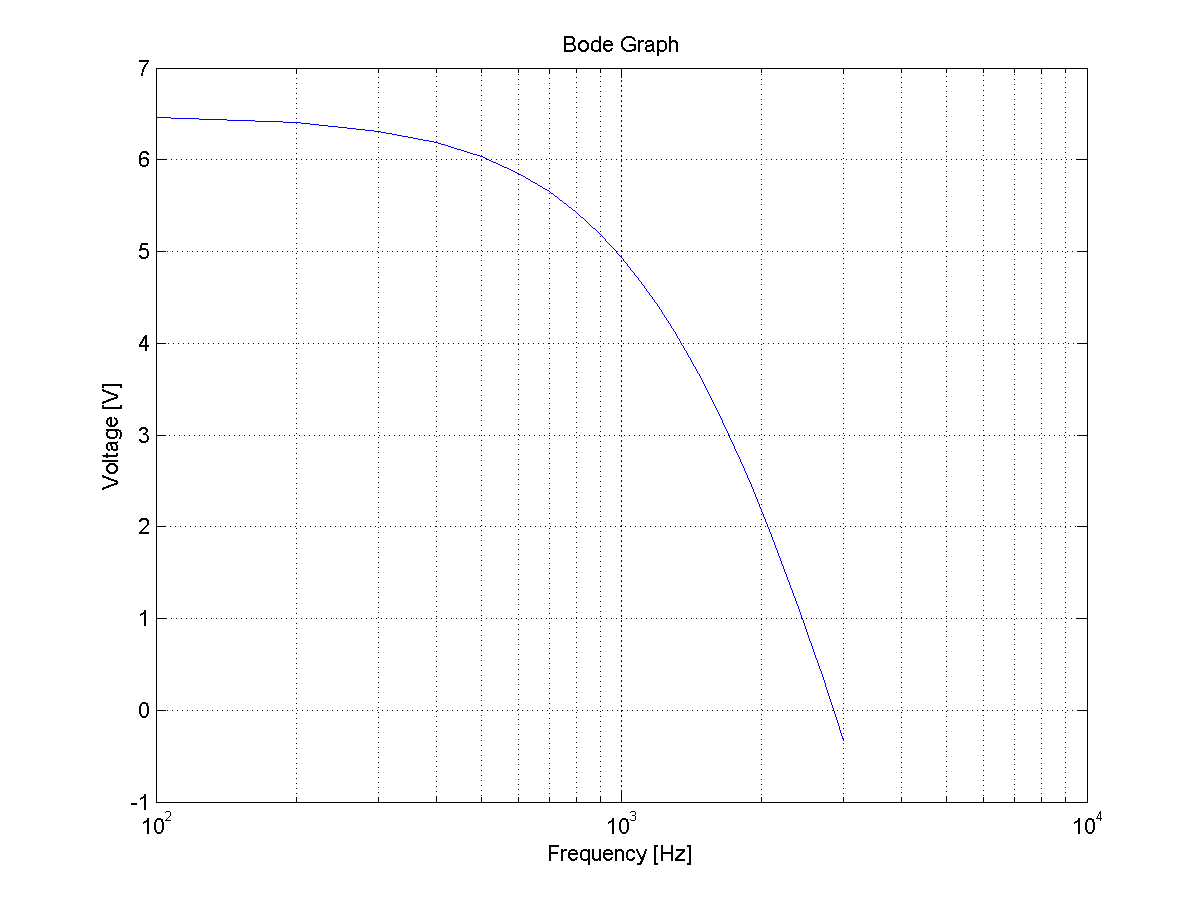
\includegraphics[width=6cm]{Figure/bode.png}}
		\caption{Bode graph}
		\label{bode}
	\end{figure}   

\ifdefined\master
\else
	\end{document}
\fi